\documentclass[./main.tex]{subfiles}
\graphicspath{{\subfix{./Abbildungen/}}}
\begin{document}
\renewcommand{\tasktitle}{Allgemeine Chemie}
\renewcommand{\taskpoints}{3.5} %Punkte in der gesamten Aufgabe mit Dezimalpunkt, der Rest mit Dezimalkomma
\renewcommand{\taskweight}{8.7}
\aufgabenanfang
Beispiel für Suchsel
\begin{alphabetsoup}[10][10]
    \hideinsoup {1} {1} {right} {t,e,s,t}
\end{alphabetsoup}
\listofclues
Hallo hier steht Text. \par

\blindtext
\teilaufgabe{\operator{Berechne} 1 + 1.}{}
\kasten{2cm}{2.\punkte{1}}

\blindtext

\teilaufgabe{\operator{Benenne} die folgenden Strukturen.}{}
\kasten{5cm}{
\begin{align*}
\punkte{2}\kommentar{Test}
\end{align*}
Dies ist die Antwort. Dies ist Antwortsatz 2.
}{}
\blindtext

\begin{figure}[H]
    \centering
    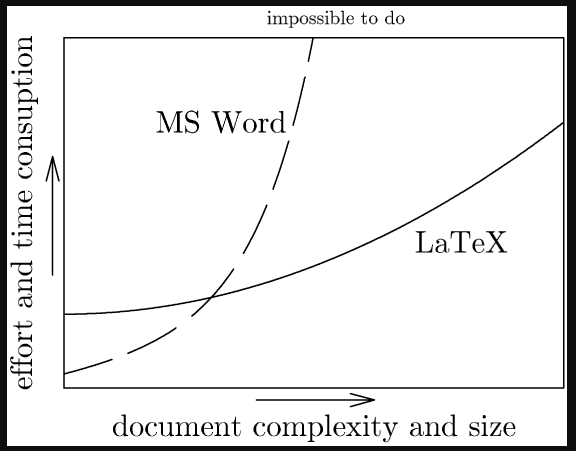
\includegraphics[width=0.7\textwidth]{test.png}
    \caption{Dies ist schlicht wahr \ldots }
    \label{A:test-Abb}
\end{figure}

In Abbildung \ref{A:test-Abb} ist das und das dargestellt \ldots 

\begin{align}
    pV &= nRT \label{G:test-Gl}\\
    a &= b
\end{align}
\textit{Hier soll kursiver Text stehen}.
In Gleichung \ref{G:test-Gl} ist das ideale Gasgesetz gezeigt \ldots 

Im Text sollten Vorzeichen wie bei $\delta-$/$\delta+$ besser au\ss{}erhalb des Mathemodusses stehen, aber ein richtiges Minuszeichen verwenden: $\delta$+/$\delta$\textminus{}

Hier kommt mal eine andere Aufz\"ahlung
\begin{enumerate}[(i)]
    \item Hallo
    \item Tsch\"uss
\end{enumerate}
Und danach wieder eine Teilaufgabe.
\teilaufgabe{\operator{Unterscheide} die verschiedenen Aufz\"ahlungen.}{}

\aufgabenende
\end{document}
